\section{Manuel utilisateur}
%\label{p2}
Le programme est utilisable en deux versions : Une première non-interactive en ligne de commande, et une seconde interactive graphique.
\subsection{Interface en ligne de commande}

Le programme peut être invoqué avec 3 arguments différents. L'abscence de arguments renvoie une erreur et un rappel sur la syntaxe des arguments attendus.

-d <folder1> <folder2> ... : Ajoute les dossiers folder1 folder2 ... à la base de données, c'est-à-dire recherche récursivement tous les ODT présents dans ces dossiers, extrait et analyse leur contenu et enregistre les titres pour une recherche future.

-f <file> : Affiche les informations importantes de l'ODT file : Chemin, titres.

-w <words> : Retourne les ODT les plus pertinents en fonction des mots recherchés. Si un "+ " est envoyé, la recherche se fera en mode ET (ie. on cherchera un ODT contenant tous les mots spécifiés après le +). Si un ensemble de mots est spécifié entre guillemets, le programme ne retournera que des ODT contenant exactement la phrase entre guillemets.

\newpage
\subsection{Interface graphique}
 \begin{figure}[!ht]
	\center
	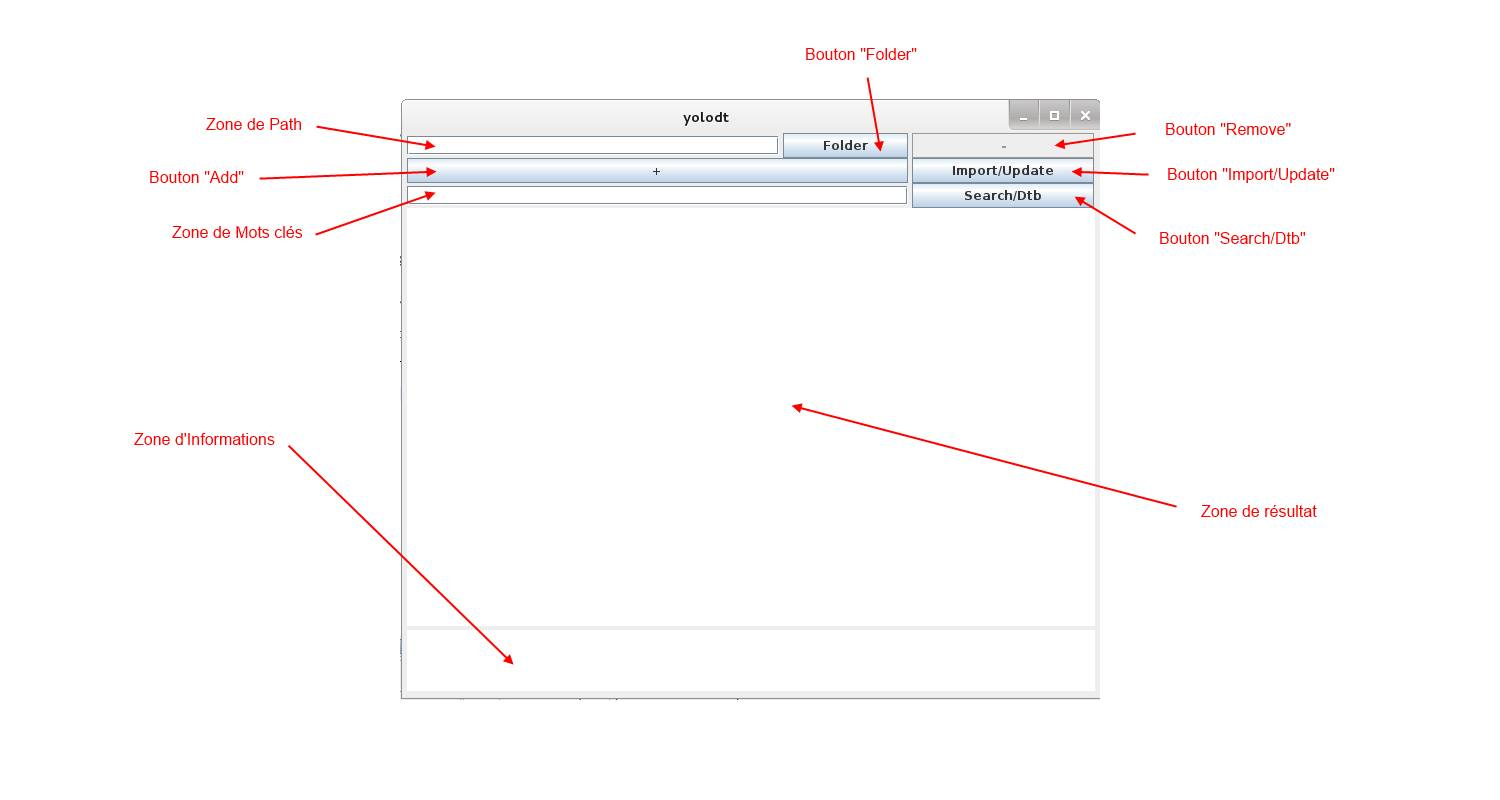
\includegraphics[width=\textwidth]{./images/gui.jpg}
\end{figure}

Résultats : L'affichage des résultats se fera dans la Zone de Résultat. 
Pour accéder a un résultat, vous pouvez double cliquer dessus au le sélectionner et appuyer sur la touche "Entrée".

Informations : L'affichage d'informations se fera dans la Zone d'Information

Zone de Path : La Zone de Path est située en haut à gauche de l'écran. Pour y ajouter plus de path, cliquer sur le bouton "Add". Pour en enlever cliquez sur le bouton "Remove". 
S'il ne reste qu'un champs, il ne peut être enlevé.

Zone de mots clés : Cette sert pour la recherche par mots clés. Mettre les mots clés recherchés séparés par un espace. Vous pouvez leurs appliquer les opérateurs suivant :
-> Si le premier mot est un "-", l'opérateur OU sera appliqué (les mots seront indépendant les uns des autres.)
Cette opérateur est utilisé par défault si le premier mot n'est ni "-", ni "+"
-> Si le premier mot est un "+", l'opérateur ET sera appliqué (le programme ne donnera que les fichiers contenant l'intégralité des mots)
-> Si plusieurs mots sont entouré par des guillemets (exemple : "Le fichier"), cela ne sera considéré que comme un unique mot

- Pour Mettre à jour la base de données :
--> Insérer les dossiers voulu dans la Zone de Path (cf Zone de Path) puis clicker sur le bouton "Import/Update"

- Pour afficher la base de données entièrement : Clicker sur le Bouton "Search/Dtb" en laissant les champs vides.

- Pour rechercher des mots dans l'intégralité de la base de données : Clicker sur le Bouton "Search/Dtb" après n'avoir rempli que la Zone de Mots Clés (cf Zone de Mots Clés)

- Pour afficher les fichiers ODT d'un ou plusieurs Path en particulier, Clicker sur le Bouton "Search/Dtb" après n'avoir remplie que la Zone de Path (cf Zone de Path)

Pour rechercher des mots dans les fichiers ODT d'un ou plusieurs Path en particulier : Clicker sur le Bouton "Search/Dtb" en ayant remplie la Zone de Path (cf Zone de Path) et la Zone de Mots Clés (cd Zone de Mots Clés)
